\documentclass[11pt, a4paper, twoside]{article}
\usepackage[latin1]{inputenc}
\usepackage[T1]{fontenc}
%\usepackage{dsfont} %double dashed fonts%
\usepackage[english]{babel}
\usepackage[pdftex]{graphicx}
\usepackage{color}
\usepackage{subfigure}
\usepackage{listings}
\usepackage[colorlinks]{hyperref}
\usepackage[small]{caption}
\usepackage{amssymb}
\usepackage{amsmath}
\usepackage{amstext}
\usepackage{tikz}
\usetikzlibrary{arrows,decorations.pathmorphing,backgrounds}
\usepackage[hmarginratio=1:2,vmargin=1in]{geometry}
\usepackage{fancyhdr}
\pagestyle{fancy}

\newcommand{\e}{\mathrm{e}} % exponential e
\renewcommand{\d}{\mathrm{d}} % for derivatives
\renewcommand{\vec}[1]{{\boldsymbol #1}}
\newcommand{\dd}[2]{\frac{\d #1}{\d #2}}
\newcommand{\pd}[2]{\frac{\partial #1}{\partial #2}}
\newcommand{\degr}[1]{$#1\,^\circ\mathrm{C}$}

\newcommand{\Rth}{R_\mathrm{th}} % to be used within $$!
\newcommand{\Ths}{T_\mathrm{hs}} % to be used within $$!
\newcommand{\code}[1]{\texttt{#1}}

\numberwithin{equation}{section} %https://www.physicsforums.com/threads/numbering-the-equations-in-latex.324808/
%\numberwithin{equation}{subsection}
\numberwithin{table}{section}
\numberwithin{figure}{section}

\title{Manual: Performance of wafer-fused VECSEL under high power operation}
\author{Stefan Keller}
\date{\today}

\begin{document}
\maketitle
\fancyhead[LE]{Manual: VECSEL high power performance}
\fancyhead[LO]{\leftmark}
\fancyhead[R]{Stefan Keller}

\begin{abstract}
\code{github.com/stefantkeller/VECSELsetup}
\end{abstract}

%\newpage
\tableofcontents\newpage

\setcounter{section}{-1} % start with 0.
\section{Refresher}

This section is for
if your computer is already set up,
the measurement routine
is adapted to your needs,
and you simply want to refresh
your memory how to get (re)started.

\begin{enumerate}
  \item record a measurement with \code{routine\_measurement.py} \\
         i.e. adjust the variables \code{samplename}, 
         \code{path\_to\_meas\_folder}, \code{heatsink\_start},
         \code{pump\_end}, \code{use\_spectrometer},
         \code{shuffle\_pump} \\
         (as explained in section~\ref{sec:routine})
  \item calibrate the setup with \code{routine\_calibration.py} \\
         If you still have a valid calibration you can skip this.
         But if you didn't measure for a while, you probably want to recalibrate!
         (as explained in section~\ref{sec:calib})
  \item evaluate the measurement with \code{light\_light\_to\_file.py}
         specify the path to the measurement logfile \code{logfile}
         and the path to the calibration data \code{calib\_folder}.
         This script returns a file that you can open for example with Excel;
         the top row states all sorts of information,
         what were the measurement conditions,
         and what the columns mean at all.
\end{enumerate}


\section{Introduction}

\subsection{Installation}

Find this documentation
and the scripts it refers to
at \code{github.com/stefantkeller/VECSELsetup}.

This is a Python library.
If you don't have Python installed yet,
I recommend you install ``Anaconda'' (\code{http://continuum.io/downloads})
for Python 2.7 (it's free!).
Also,
you have to have installed
the drivers from National Instrument (\code{ni.com}),
in order to communicate with GPIB
(etc\ldots (NI drivers are a mess, what exactly you need, you have to figure out yourself)).

To install this library
from github,
\begin{enumerate}
  \item click on ``Download ZIP'',
  \item extract the .zip
  \item copy the folder to where ever you want it
  \item adjust the PYTHONPATH
\end{enumerate}
(at least, that's the proper way to do it, I guess).  
And, if you are familliar with git \ldots you know what to do.

If you don't care about ``proper''
and you simply want it to work
(I don't know though what this breaks along the way\ldots):  
after extracting the .zip,
copy the folder to (something like; if you work with Anaconda as recommended above)
\begin{itemize}
  \item Windows: \code{C:\textbackslash Anaconda\textbackslash Lib\textbackslash site-packages}
  \item Mac: \code{/Users/yourusername/anaconda/Lib/python2.7/site-packages}
\end{itemize}
this path is already in the Pythonpath,
and Python will find it.

For measurements (the stuff in \code{meas/}) you need pyvisa \\
(\code{https://pyvisa.readthedocs.org/en/master/}).\\
For evaluation (the stuff in \code{eval/}) you need to also install errorvalues \\
(\code{https://github.com/stefantkeller/errorvalues}). \\
Install it with the same procedure as listed above.
If you intend to use the calibration in \code{exp/eval/calibration.py} as it is,
this is going to write an automated report (tuck together some plots) as a pdf;
ready for print.
This relys on \LaTeX (\code{pdflatex}) to be installed on your system.

If measurement and evaluation happens on two different computers (recommended)
you probably install only those dependencies that you need.
That's ok, the error handling in \code{\_\_init\_\_.py}
catches \code{ImportError}s and ignores them.
However, if nothing happens at all,
you might want to check whether you have installed,
what you're supposed to have installed
(maybe everything is caught and subsequentially ignored?).

\subsection{File hierarchy}

The different folders have different purposes:
\begin{itemize}
  \item meas, setup control to record measurements
  \item eval, scripts for evaluation of measurements
  \item exp, examples of working measurement routines (using meas), and evaluation (using eval)
  \item doc, documentation
\end{itemize}

\subsection{Usage}

Copy the files stored from the folder \code{exp} in your working directory.
The example \code{exp/meas/routine\_measurement.py} is the most exhaustive for setup control / recording measurements.
While \code{exp/eval/light\_light.py} highlights the evaluation part.

There is not graphical user interface (GUI),
as one might know from LabView.
Instead, with this library
you have full controll over
what the software does.
But this comes with the price
to actually having to read the lines of code --
instead of looking at obscure icons.
There are only few lines of code
to read,
in order to understand what's going on;
and those are accompanied with comments.
So go ahead and read it.
You best start with the example scripts in the folder \code{exp}.

These lines of code
you can read with any text editor
of your choosing.
On Windows I recommend PyScripter (\code{https://code.google.com/p/pyscripter/}).
It brings in some simple GUI features,
so you can edit and launch your measurement routines easily,
see Fig.~\ref{img:pyscripter}.

\begin{figure}
\centering
\subfigure{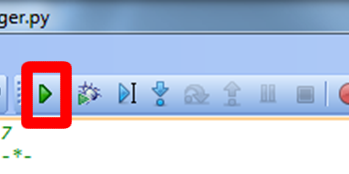
\includegraphics[width=4cm]{img/pyscripter_launch.png}}
\subfigure{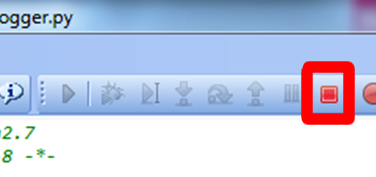
\includegraphics[width=4cm]{img/pyscripter_stop.png}}
\subfigure{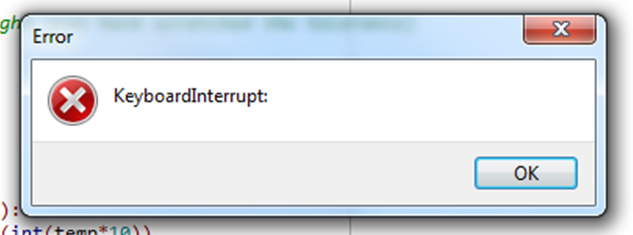
\includegraphics[width=4.5cm]{img/pyscripter_ki.png}}
\caption{PyScripter is a convenient tool
to work with python scripts.
When you have opened one of the examples
from the folder \code{exp/}
you can simply click on the launch button,
the scripts starts and
writes the output in one of the subwindows --
try it out, should be selfexplanatory.
The stop button
lets you to interrupt the script if required.
For example, \code{exp/meas/temp\_logger.py}
logs the heat sink temperature in an infinite loop;
in order to stop the logging you have to interrupt it.
This interruption raises a \code{KeyboardInterrupt} error.
This is supposed to happen.}
\label{img:pyscripter}
\end{figure}

\subsection{Disclaimer}

Some paragraphs in this documentation
are copy-paste from the master project report,
during whose period the presented scripts
have established themselves.
A back-up copy of said report
you will find at \\
\code{github.com/stefantkeller/VECSELMasterProjectReport}.

\section{Measurement Routine}
\label{sec:routine}

The routine is written in Python.
This brings in several advantages:
First of all we can actually look through the code
and comment on it,
where clarification is needed.
The Python syntax is simple enough --
basically, English with peculiar grammar --
so if you can read this documentation,
you will understand the program just as well.
LabView for example
fails at exactly this point;
it's very hard to maintain,
and the different sections
of the script are difficult to interpret
(let alone the litteral spaghetti code).
And lastly,
with Python we don't depend on a third party license.
Again, LabView and Matlab
fail at this point.

\subsection{The routine}
\label{sec:routine:routine}

You either look at the example
given in ``exp/eval/routine\_measurement.py''
and read it through,
or you continue to read here.
The following long text covers the same.

We choose a set of values corresponding to
a) the current of the pump laser,
and b) the temperatures of the heat sink.
We specify further, a path where to store the results.
And lastly, we choose on how often every power current
is ought to be measured --
repeated measurements in order to obtain
the errorbars
that inform us on the reliability of the results.

At each temperature,
we set the power source to the requested currents,
and read out the power meters.
The results of each power meter is written in its own file.
Each of these files starts with a header line,
that contains the state of the relevant settings of the device in question.
Consequentially,
if we doubt the integrity of the measurements
we can look at this header line and
at least know what state the device has reported to be in.
The information about the power source
are also written to its own file,
containing the set and actual current.
Hence, at each temperature we generate
one file for the power source, plus one for each power meter.

At the end of these measurements we write a line in a logfile:
The set temperature,
the actually reached temperature,
the filenames of the files
with the results of the different devices,
along with a timestamp so we know which measurement took how long.
The timestamp also allows us to connect certain effects
to the time of the day it was measured.
The approach with a logfile
and the separate files of each device
(whose names are automatically stored in the logfile),
facilitates the analysis;
all the information a analysis-script needs is specified in the logfile.

At each heat sink temperature
we irradiate the sample
with different pump powers.
Each pump is repeated $N$ times over all.
The pump order is selected at random,
as illustrated in Fig.~\ref{img:random_sampling}.
Thanks to the random sampling
the measurement results
are detached from the lab environment --
most notably time-independent.
The heat sink cannot control its temperature
with absolute precision.
Figure~\ref{img:random_sampling_heatsink}
illustrates this issue:
It shows
the actually present heat sink temperature
for six set temperatures.
In the left column
the temperatures are plotted
in chronological order.
We can identify,
the temperature drifts.
The right column shows the same temperatures,
but corresponding to the set pump.
The repeated measurements
see a spread of different temperatures
but the temporal drifts can not be resolved.

In contrast,
Fig.~\ref{img:random_sampling_ramp_heatsink}
shows the heat sink temperature
during a measurement without the random pump selection.
In this case, clearly,
we cannot talk about a single heat sink temperature
for all the pump settings
for this specific set heat sink temperature.
The resulting measurements are highly repeatable,
but only given the same pump order.
This pseudo-stability
we exploit
during the calibration process
of the different beam samplers
and detectors:
During the calibration
we don't care about reproducibility
but solely about the repeatability
of two consecutive measurements.

\begin{figure}
\centering
\subfigure{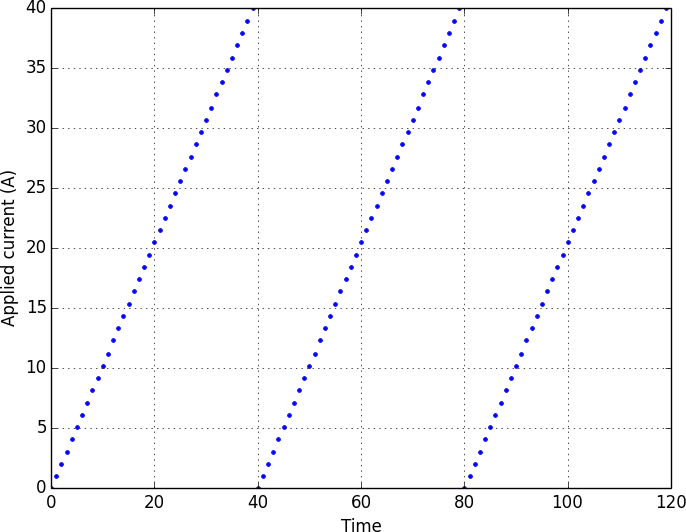
\includegraphics[width=7cm]{img/random_sampling_ramp.png}}
\subfigure{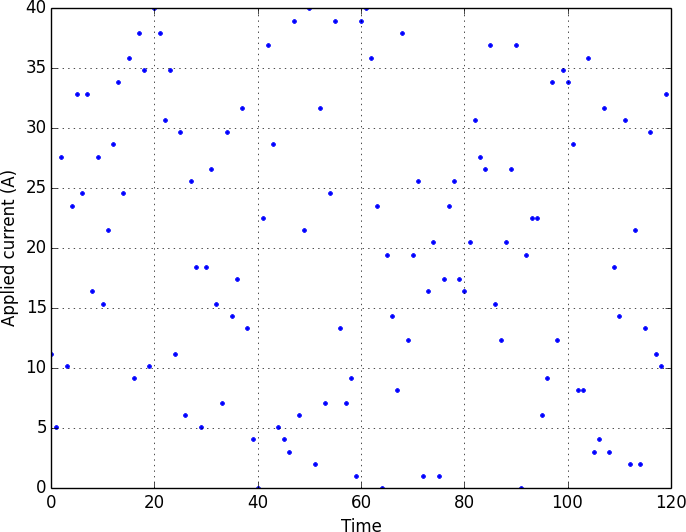
\includegraphics[width=7cm]{img/random_sampling_random.png}}
\caption{Two examples to apply various pump settings, with a repetition rate of 3.
Left: A ramp. Right: Random sampling.}
\label{img:random_sampling}
\end{figure}

\begin{figure}
\centering
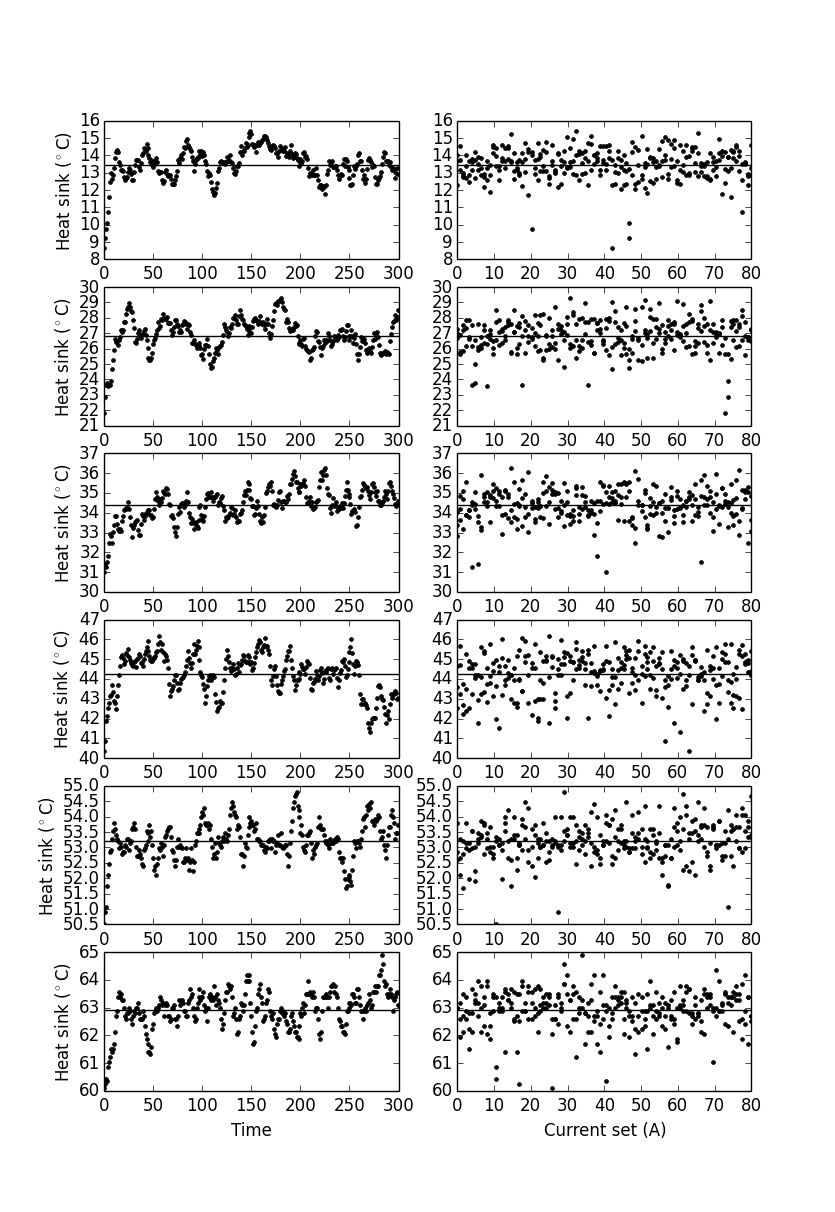
\includegraphics[width=15cm]{img/random_sampling_heatsink.png}
\caption{The heat sink temperature fluctuates over time (left).
Thanks to the random sampling addressed in Fig.~\ref{img:random_sampling}
the measurements don't see these drifts (right).}
\label{img:random_sampling_heatsink}
\end{figure}

\begin{figure}
\centering
\subfigure{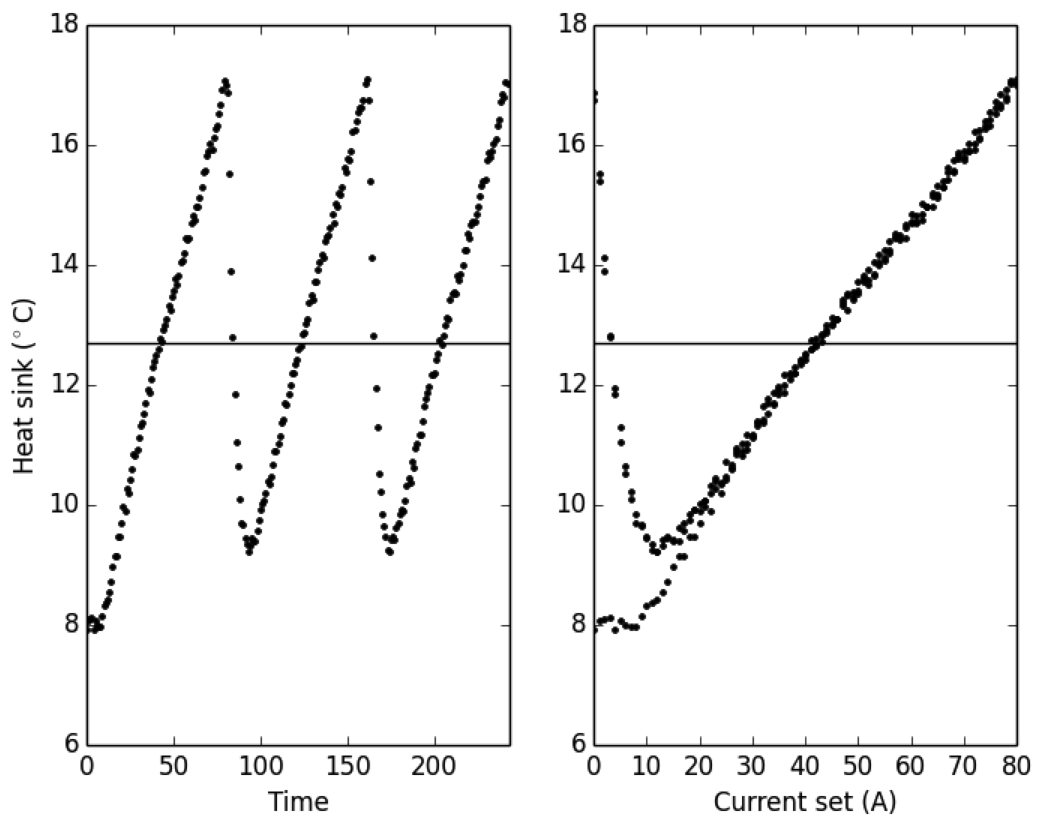
\includegraphics[width=7cm]{img/random_sampling_ramp_heatsink.png}}
\subfigure{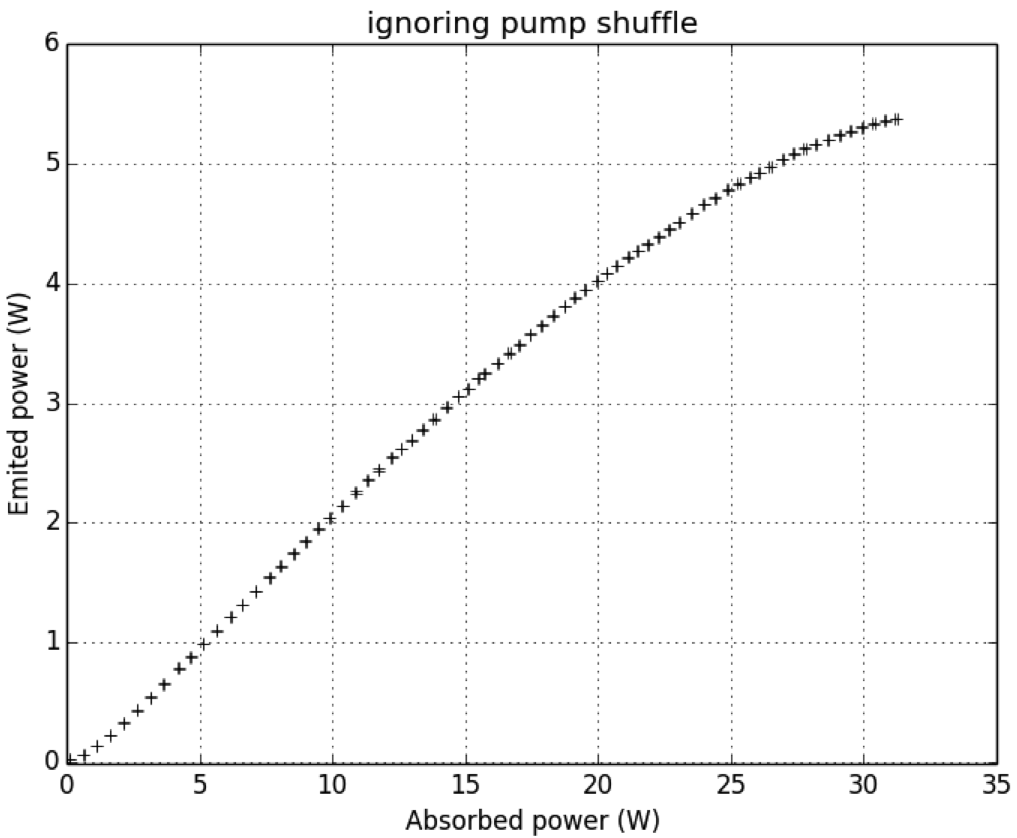
\includegraphics[width=7cm]{img/random_sampling_ramp_noisfreeLL.png}}
\caption{In contrast to Fig.~\ref{img:random_sampling_heatsink},
when we ignore the random pump sampling
highlighted in Fig.~\ref{img:random_sampling},
the temperature seen by the single pump settings
differ strongly from the average heat sink temperature
(left).
The resulting LL-characteristic
has very little noise on its data points
(right).
But these small error bars dismiss the fact
that the underlying points were measured
under very different conditions;
eroding the significance
of this low noise.}
\label{img:random_sampling_ramp_heatsink}
\end{figure}

The power meter average each measurement point
over 200 samples,
of which each one sample
takes approx. 3 ms \cite{ThorlabsPM}.

The order of heat sink temperature
is still a ramp:
I expect the setting of a new temperature to be somewhat time consuming.
Therefore, we want to make use of the previously set temperature.
The measurement routine looks at the specified temperature range,
picks the one closest to room temperature,
and increases to every second entry.
Once the highest temperature is reached,
the residual temperatures are picked,
in descending order, until the lowest temperature is reached.
From there we heat back up to room temperature.
This routine is illustrated in Fig.~\ref{img:temproutine}.

\begin{figure}
\centering
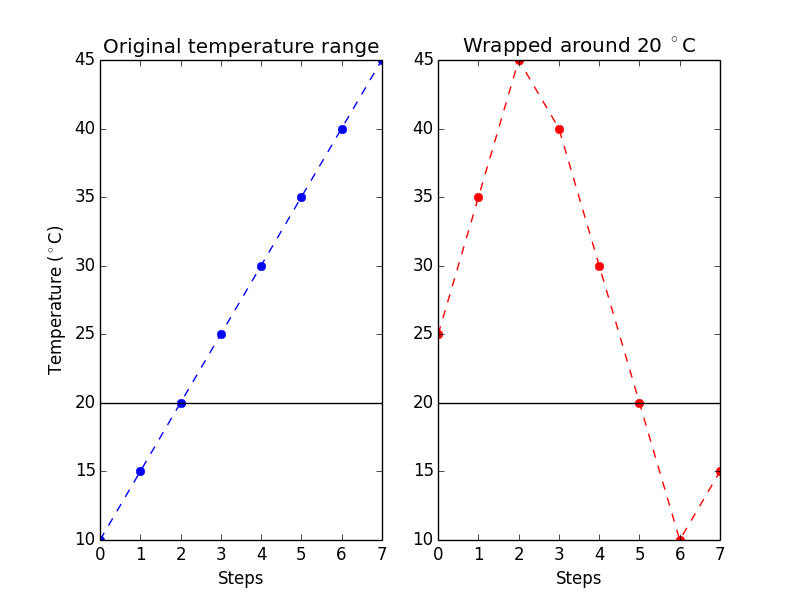
\includegraphics[width=12.5cm]{img/temp_wrap.png}
\caption{An example of how a given temperature range is wrapped around the room temperature
(here assumed to be \degr{20}).}
\label{img:temproutine}
\end{figure}

As mentioned already,
we repeated the measurement of each pump setting
$N$ times.
With this repetition we obtain a measure
for how well we know
the underlying true value.
We are hence interested in
the mean of these single measurements and
the resulting unbiased standard error \cite{Barlow}
\begin{equation}
\Delta x = \sqrt{ \frac{1}{N(N-1)}
	\sum\limits_{i=1}^N (x_i - 
		\frac{1}{N} \sum\limits_{i=1}^N x_i )^2 }.
\label{eq:sterr}
\end{equation}

For the uncertainties attached to
quantities obtained through fits,
I use a so-called
Jackknife \cite{Efron1983} approach:
In a nutshell,
this method allows to estimate
the influence of the single measurement points
on the fit parameters
without working through
the covariance matrix of the fit.
The resulting error value
is directly related with the
unbiased standard error (\ref{eq:sterr}),
used for the rest of the report.

\subsection{Safety precautions}
\label{sec:routine:safety}

The goal of this script is to automate as much as possible.
Ideally,
we want to install a new VECSEL,
align the output coupler,
press start,
and return some time later to a complete data set
for this specific VECSEL under test.
For this we need to be sure
our measurement routine handles potential errors appropriately.

For this we must not rely on software.
Instead, we have to implement the safety precautions on hardware side.
In software we can try to mitigate
potential problems through proper error handling.
I don't know how this would be done in LabView.
In Matlab and Python this is performed through so-called
try/catch and try/except handles, respectively.
With it I have implemented that if anything goes wrong software side,
the power source is shut down
(This order itself is so low-level,
that it \textit{should} always work.).
For example, one of the devices could send an unexpected answer,
the heat sink doesn't reach its requested temperature within reasonable time, etc.
For the unlikely event
that even the power source shut down doesn't work,
we have to implement the safety precautions on hardware side.

Our power source has two ways to be shut down:
We can disable the current,
or we can set the current to zero.
In order to disable the current,
we first have to ask the power source,
whether the current is currently applied.
If it is, we toggle it like a light-switch to shut off.
However, querying the current state
is error-prone.
Hence, if an error is caught we leave the shutter to be in what ever state it is
and only set the current to zero.
Potentially it is still applied.
But the light output at $0\,\mathrm{A}$
is barely detectable --
but there still \emph{is} a leak flow of photons.
Writing to the power source should not cause any new problems,
so simply writing $0\,\mathrm{A}$ should go through.

On the hardware side,
the ``laser on'' light in front of the lab
is controlled by a logic tied to the power source:
As soon as the power source applies a certain specified voltage
the laser warning turns on.
During the measurements this safety sign therefore
is always on.

As a second safety precaution I supply a script that allows us to test 
modifications on the measurement routine with fake devices.
In order to connect the measurement routine with the measurement devices
we have to specify a protocol.
In the new script we do this by selecting an external file
that contains the initiation details.
By specifying the fake protocol we can modify the routine without the real devices.
This separation in code is, for one, good practice,
and secondly convenient if we cannot use one of the devices due to a revision or whatever.
To be detached from the physical devices was not possible with the old script --
which is one of the reasons why it was possible to toggle the power source shutter
while setting the wavelength of the power meter.


\section{Calibration}
\label{sec:calib}

\begin{figure}
\centering
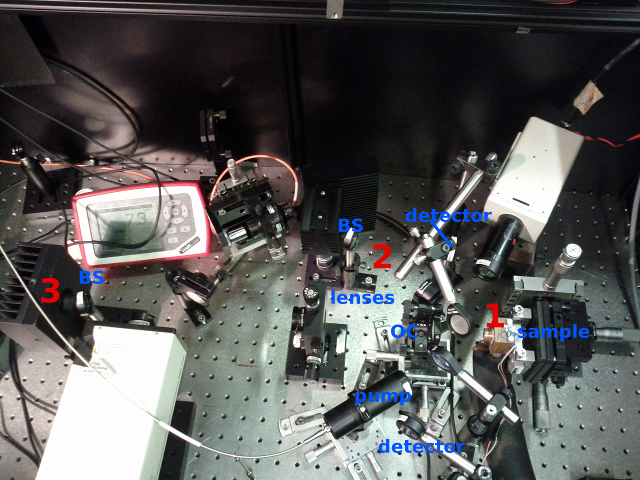
\includegraphics[width=12.5cm]{img/calib_setup.png}
\caption{In order to calibrate the setup we have to
measure the actually present power at the indicated positions 1--3.}
\label{img:calib_setup}
\end{figure}

Figure~\ref{img:calib_setup} shows a photograph of the setup.
Before we can use it to characterize samples,
we have to characterize the setup first.
Following the beam path,
we start with the lens system indicated as pump.
This input beam is targeted at the sample.
Part of this pump beam is sampled by a beam sampler (BS),
a glas plate with high damage threshold and
anti reflective coating on one side.
This sampled light is directed towards a detector.
The pump light is reflected off the sample,
collimated by a lens,
and again sampled as for the input.
The lasing output passes the output coupler (OC),
a collimating lens,
and another beam sampler (coated for the emission wavelength).
This beam sampler we eventually use to record the spectrum of the emission.

In order to calibrate this setup we need to know
how to correlate the readings of the single detectors
with the actually present powers.
For this we place the thermal power meter at
the four indicated positions.
With the thermal power meter we can validate
the setup up to $40\,\mathrm{W}$, in principle.

Position 1 requires to remove the sample.
We're interested in the correlation between the readings
of the detector after the beam sampler
and the measurements at the sample position.
From this same measurement we can also extract
a look-up-table what current setting of the pump laser
corresponds to what output power.

On position 2 we measure the beam power present after the collimating lens.
This we relate with the readings of the detector after the beam sampler
gathered during the measurements of position 3 and 4.
As I realized after the measurement I should have removed the lens as well --
we want the reference value to correspond
to the power before beam sampler
and lens.
In order to calibrate the reflection detector
we combine the results from two different measurements.
Between these two measurements we don't change
any of the elements within the beam path.
Non the less,
calibrating the reflection detector
relies on the repeatability of the operation.
To keep track of this repeatability
we measure each pump setting
multiple times --
3 times for the presented data,
each within a random order,
see section~\ref{sec:routine}.

The measurements taken at position 3
(with the lens removed,
reading out the output directly after the output coupler)
and position 3
(the real position of the power meter during regular operation)
allow us to infer from the results obtained
at position 4 to the undistorted output power.



\section{Measurement alignment process, description of}
\label{sec:alignment}

\begin{figure}
\centering
\subfigure{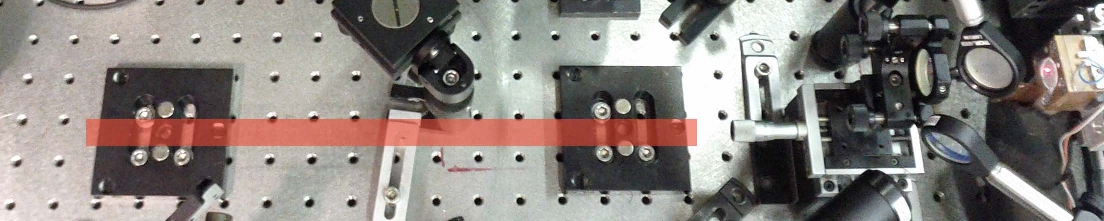
\includegraphics[width=10cm]{img/beamline_empty.jpg}}
\subfigure{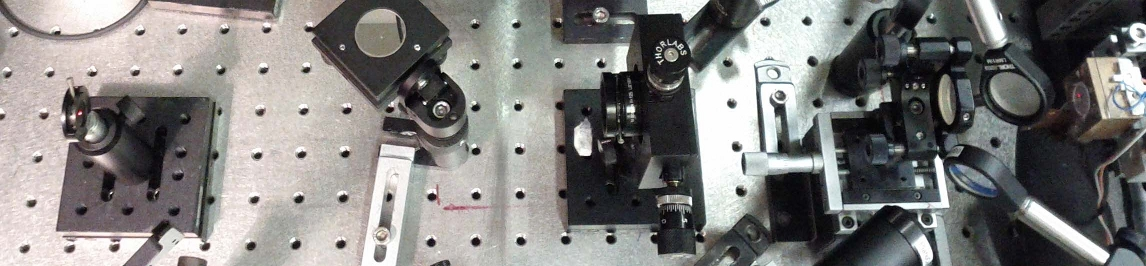
\includegraphics[width=10cm]{img/beamline_populated.jpg}}
\caption{Top: Removeable posts to define the beamline.
Bottom: HeNe beam has to be directed through the two irises.
With these two irises the position of the HeNe source is detached from the beam line.}
\label{img:beamline}
\end{figure}

The alignment process comes in two steps:
a rough base alignment
and a fine tuning.
For the first step
align the optical elements
along the emission path
to be orthogonal to it.
With the equipment
orthogonal to the beam path
we arrive
at a well-defined state,
which is easy to reproduce.

First we define the beam line.
It is defined by
two removable magnetic posts,
Fig.~\ref{img:beamline}.
These posts allow us to remove and replace a mount reproducible.
Two irises
define the beam line height.
This height
is arbitrary,
but in order to have
a reproducible setup
pick a height
and use this iris
as a reference tool.
Use the HeNe laser
for the rough alignment:
place it anywhere
on the table.
Send its beam
through the two irises;
using mirrors.
The two irises
are all we need
in order to define
the beam line.
With them
the setup is detached from the rest
of the table.

Place the sample
on the heat sink
and align it
orthogonal to the aforementioned beam line:
Remove -- or flip, Fig.~\ref{img:cavity_flipped} --
all other components along the beam line
and leave only the sample.
Adjust the orientation of the sample such that
the back-reflection is directed at the HeNe, Fig.~\ref{img:HeNe},
now it is in a well-defined configuration.
Once the sample is aligned,
place the output coupler
back in the beam path.
Repeat the same procedure.
Careful:
since the output coupler is curved
you will find two reflections.
One looks like in Fig.~\ref{img:HeNe}.
This you can align by tilting
the output coupler;
like a regular mirror.
The second reflection
is divergent.
Bring it to the center
using the xyz-translation-stage.

The last equipment
in this beam line
is the lens
after the output coupler.
It -- in combination with the output coupler --
images the sample
onto the camera
you'll use later.
Align the lens orthogonal
and choose its position
with appropriate distance
from the output couper
and camera.
Appropriate means
the picture on the camera is in focus
and there is enough room
for all the equipment.

\begin{figure}
\centering
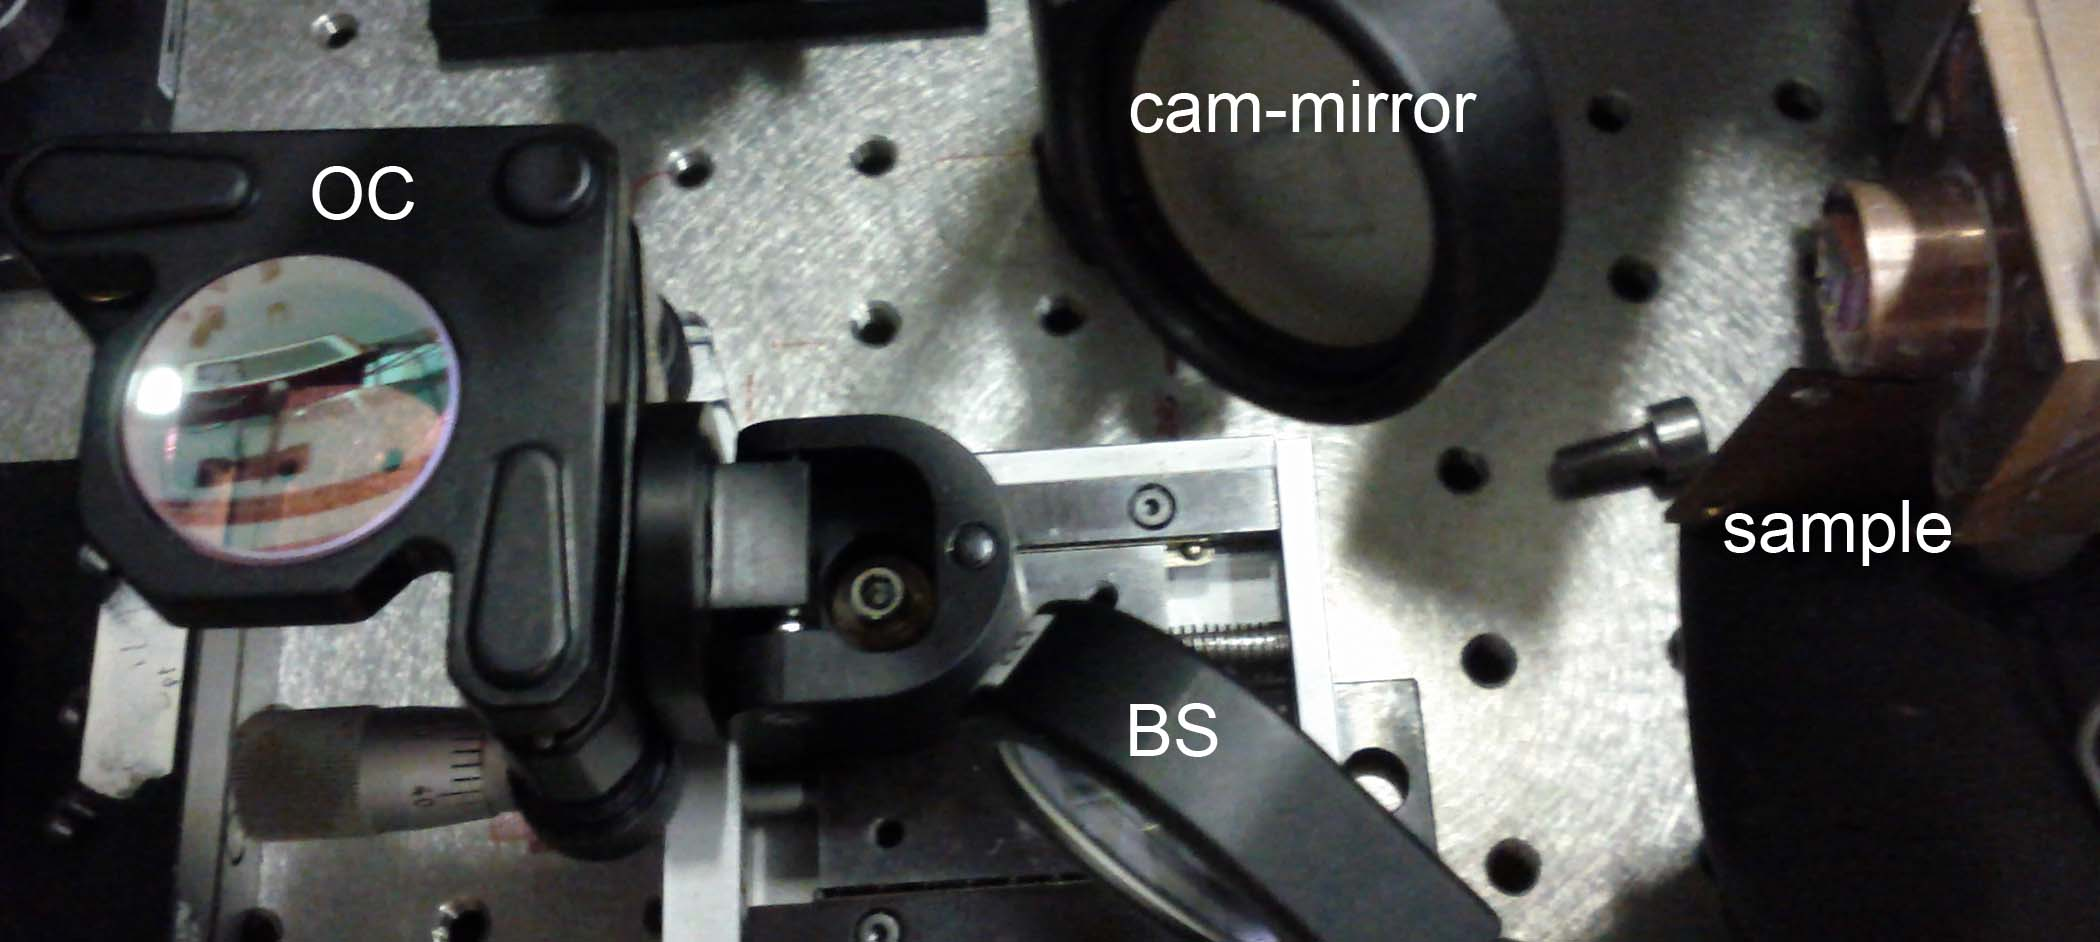
\includegraphics[width=10cm]{img/cavity_flipped.jpg}
\caption{First, we remove / flip all components along the beam line except the sample.
In this configuration we align the sample surface orthogonal to the HeNe.}
\label{img:cavity_flipped}
\end{figure}

\begin{figure}
\centering
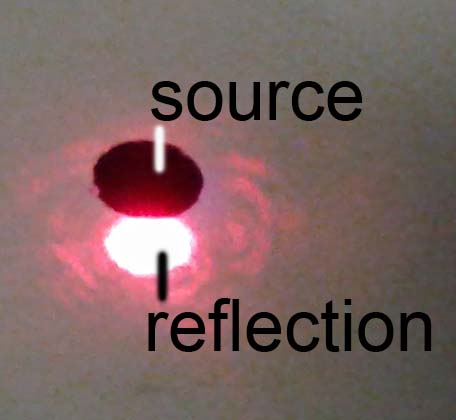
\includegraphics[width=4cm]{img/HeNe.jpg}
\caption{By arranging the reflected beam to coincide with the HeNe source position
we ensure the orthogonality of the component.
The orthogonality is an easily obtainable well-defined state,
it thus helps for reproduciblity.}
\label{img:HeNe}
\end{figure}

For the fine tuning
we need the pump light
and look at the photoluminescence
of the sample.
The camera along the emission beam line,
mentioned above,
sees the photoluminescence
resulting from the pump on the sample.
Attach a long-pass filter
to the camera
in order to see only the photoluminescence
and not the pump light.
With this camera --
initially,
thanks to the rough alignment --
we see two spots corresponding to
pump and reflection from the output coupler,
Fig.~\ref{img:spot_overlap}.
If you don't see two spots
the rough alignment
with the HeNe
was not precise enough;
repeat.
Don't forget to test whether
the sample really is
in focus of the camera.
Otherwise,
of course you won't see anything.
Bring these two spots to overlap,
using the xyz-stage of the output coupler.
Once the two spots do overlap,
and the pump is above threshold,
the sample starts lasing.
Congratulations,
the setup is aligned.

\begin{figure}
\centering
\subfigure{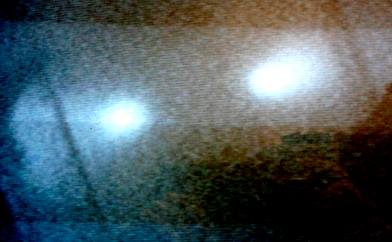
\includegraphics[width=6cm]{img/spot_overlap_two.png}}
\subfigure{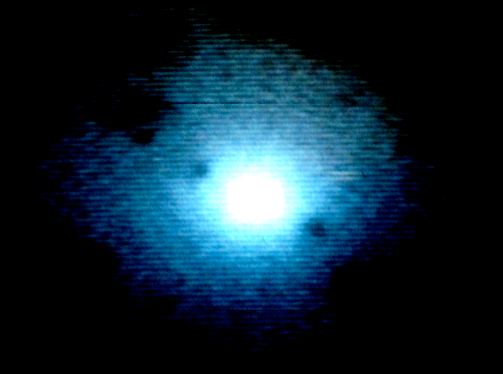
\includegraphics[width=6cm]{img/spot_overlap_one.png}}
\caption{After the pre-alignment
with the HeNe,
the two spots --
originating
from the pump
and the output coupler reflection --
are close by (left).
By optimizing the alignment
of the output coupler,
these two spots
have to be brought to overlap (right).
Given this configuration,
we have to increase the pump power,
and at threshold we obtain laser emission.
For the fine-alignment
we have to replace the camera
with a power meter
and adjust for maximum output power.}
\label{img:spot_overlap}
\end{figure}

Now you have to make sure
the beam sampler
for the pump and reflection detectors
actually send off
the sampled beam
towards the aperture
of the detectors.
If you move the pump beam sampler,
the spot moves
on the sample,
detuning the alignment
just described;
repeat.
An additional reminder
about some obvious alignment necessities:
The distance between
output coupler and sample
has to be smaller than
the radius of curvature
of the output coupler.
The distance between
pump and sample
has to match
the focal length
of the pump lens
(provided the light is collimated
after the first lens).

Figure~\ref{img:overview} shows an overview of the different components.
The pump light is directed via fiber to a lens system that images the light onto the sample.
With beam sampler BS$_p$ we extract a fraction of the pump and direct it to detector det$_p$.
This way we have a realtime reading of the pumped power.
A considerable part of the pump light is reflected off the sample.
This light diverges.
First, we thus have to collimate it.
For this we install a lens with appropriate focal length and distance from the sample.
Of this reflected beam we again sample a fraction with BS$_r$,
and direct this to detector det$_r$.
The largest fraction of the reflected beam is directed to the beam dump.
By sampling pump and reflection in this geometry
we avoid high power readings on the detectors.

\begin{figure}
\centering
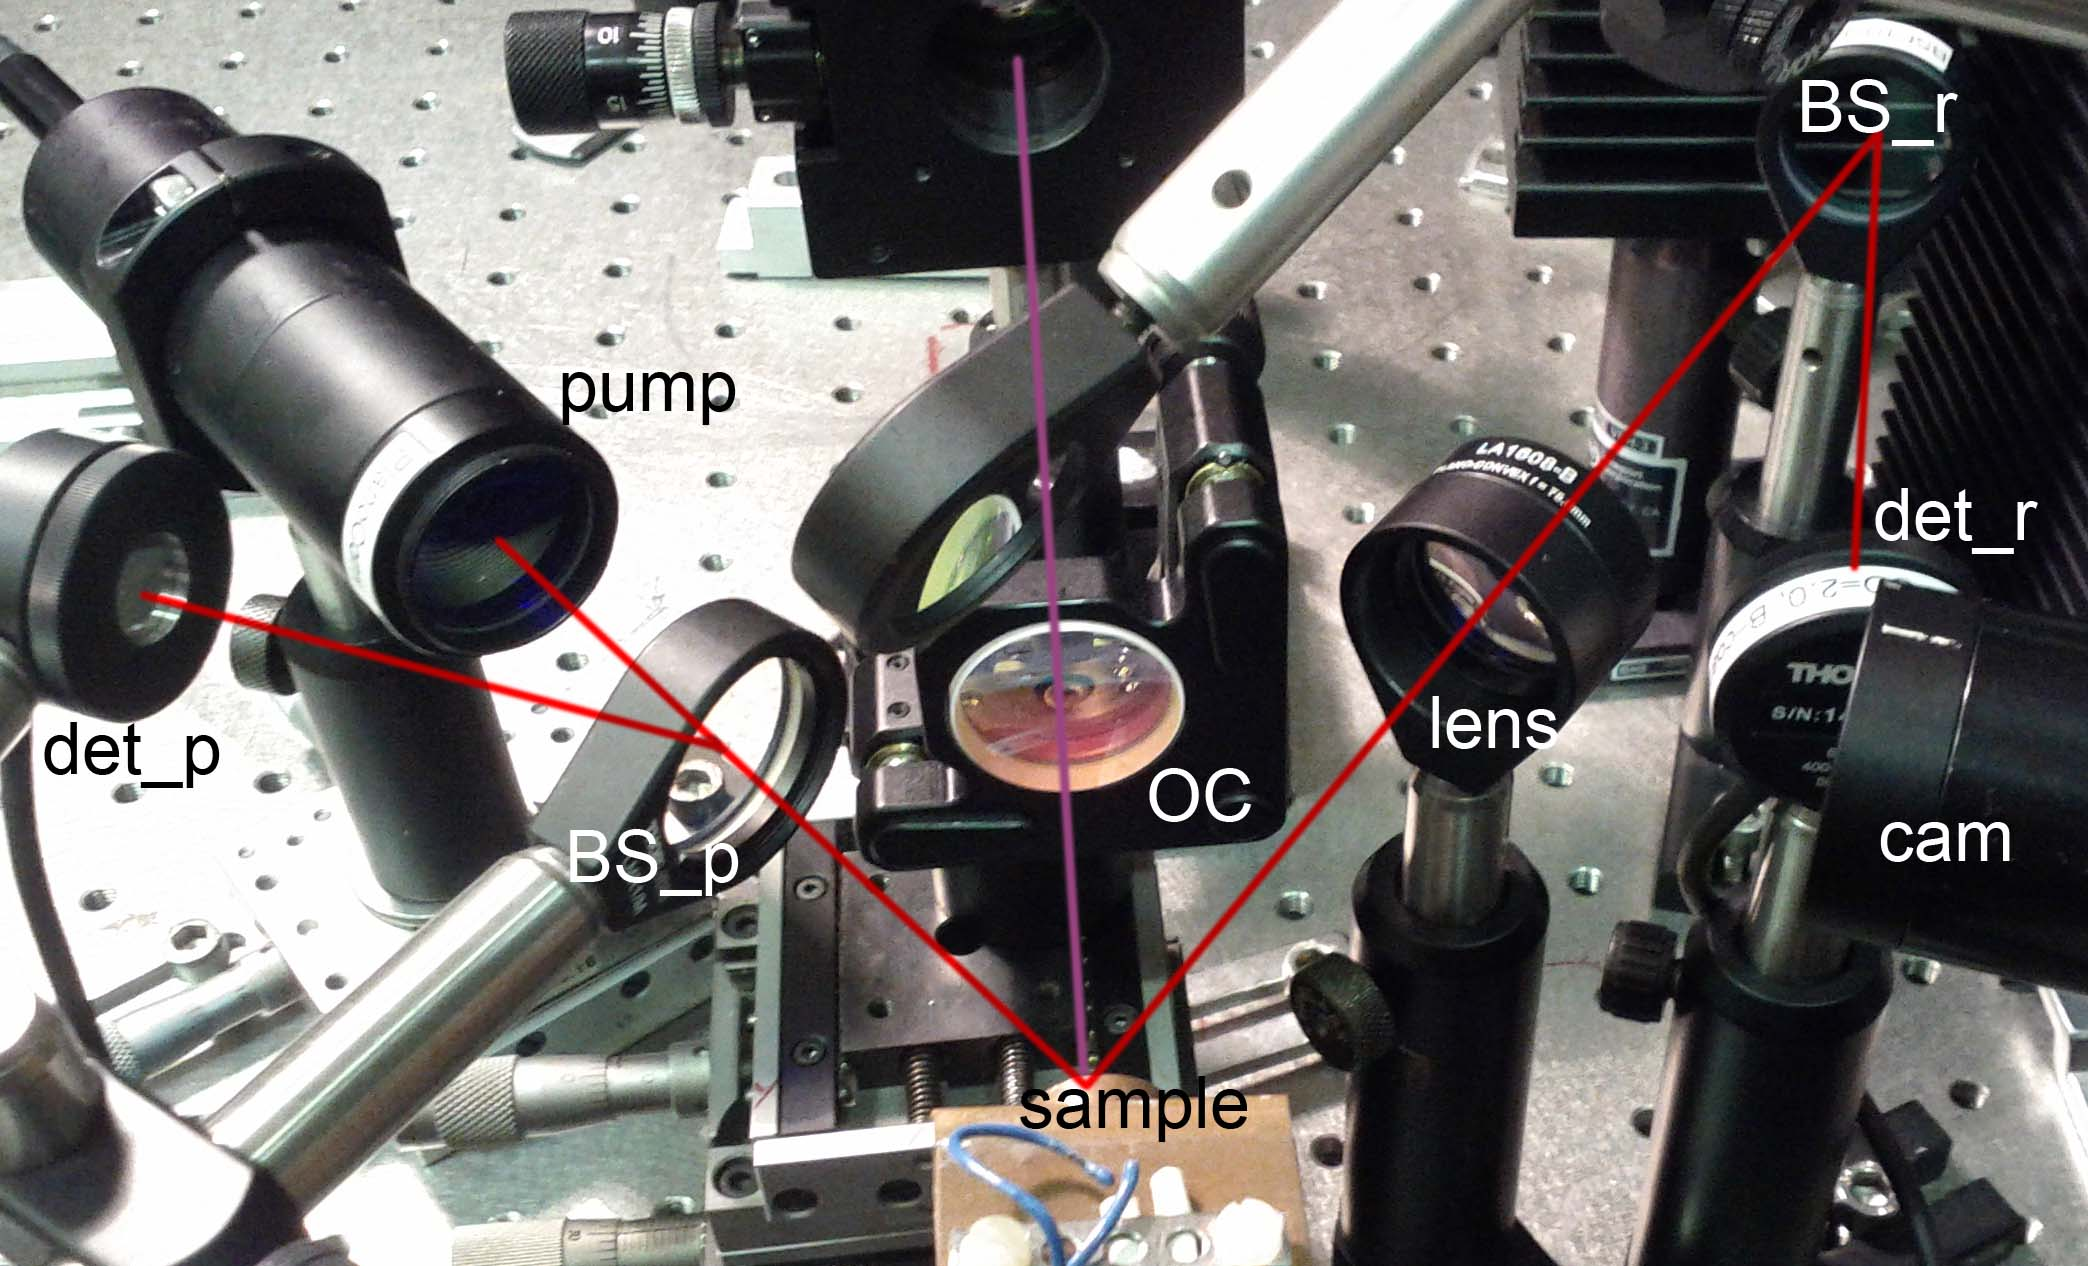
\includegraphics[width=10cm]{img/cavity_all.jpg}
\caption{Overview of the different components incorporated for the cavity.}
\label{img:overview}
\end{figure}

Before you record a measurement
you want to optimize the alignment once more:
place the power meter
in the emission path,
set the pump to a value
above threshold,
and optimize
for maximum output power.
Don't move the sample,
only adjust
the xyz-stage
of the output coupler,
and the distance between
pump and sample.
For measurements
that record the spectral information,
place also the assigned beam sampler
in the emission path.

The fiber delivering the light
to the spectrometer
is at a distance
from the sample
similar to the camera;
in the focus of the emission.
In order to have access
to both the camera
and the spectrometer
within the same setup,
several mirrors
are flippable
to use the equipment needed for the alignment step
you are at.
Coupling the emission
into the fiber
is straight forward;
but can be frustrating,
because this alignment is delicate.
You have to hit the position of the fiber core
and you have to hit
with normal incidence.
The angular component
is tricky.
We use a multimode fiber,
those allow for a larger margin of error.
Use the IR-viewer or an IR-card
to visualize the emission beam,
mount the fiber
such that is along this beam line,
and direct the beam onto the fiber.
Once you have a reading
on the spectrometer
adjust the alignment
for maximum signal.

\section{Sample surface microscopy}
\label{sec:microscopy}

Take a picture of the non-radiative defects
of the sample
under the microscope.
For this connect the pump light
with the microscope illumination,
and place the camera,
including a long-pass filter
so we see only the photoluminescence
and block the pump,
as illustrated in Fig.~\ref{img:microscopy}.

Note:
Whenever you change the fiber
connected to the pump diode,
ensure the fiber is intact --
to avoid damages portrayed in Fig.~\ref{img:burnt} --
and make sure
to have the best possible
diode-to-fiber coupling.
For the first task
use the fiber inspection microscope.
For the latter
(see diode manual!)
apply a certain pump,
unscrew the fiber connection
at the pump diode module,
and turn the fiber end
while observing the change in output power.
Lock it for the maximum configuration.

With a microscope magnification of $5\times$,
take a picture of all four corners.
For this you can use
the fully equiped NI-MAX,
which came along with the other NI drivers,
see Fig.~\ref{img:ni_max}.
The overlapping parts of these images
allow you to staple together
the whole photograph.

\begin{figure}
\centering
\subfigure{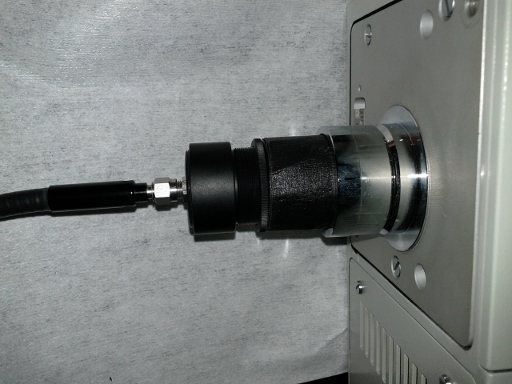
\includegraphics[width=6cm]{img/micro_illum.jpg}}
\subfigure{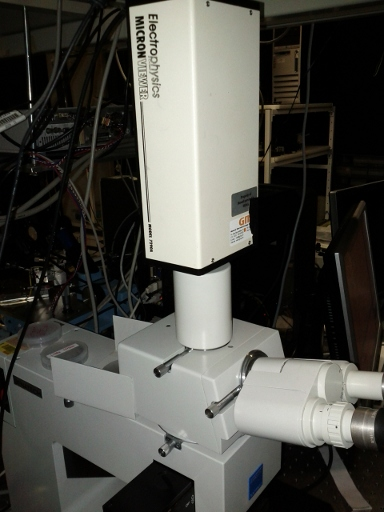
\includegraphics[width=6cm]{img/micro_cam.jpg}}
\caption{Direct the pump light to the microscope for illumination.
With this light source,
and a long-pass filter on the camera,
the non-radiative defects are directly visible.}
\label{img:microscopy}
\end{figure}

\begin{figure}
\centering
\subfigure{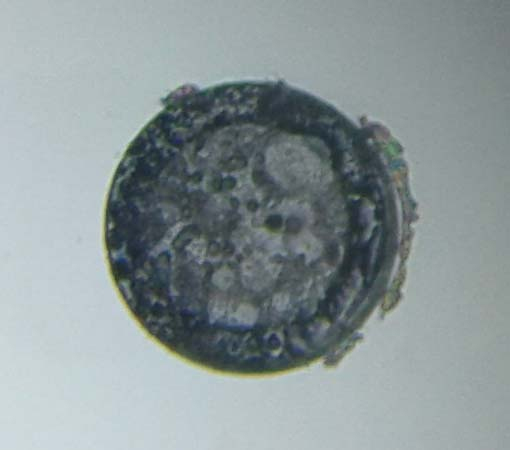
\includegraphics[width=6cm]{img/fiber_bad.jpg}}
\subfigure{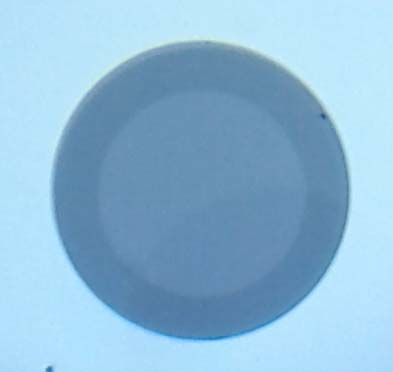
\includegraphics[width=6cm]{img/fiber_good.jpg}}
\caption{Left: This fiber end is burnt; it delivers a beam of bad quality.
Rigth: This is how all fiber interfaces are supposed like; it is intact.}
\label{img:burnt}
\end{figure}

\begin{figure}
\centering
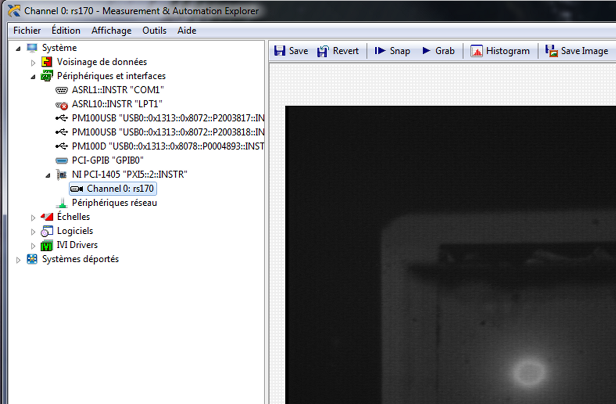
\includegraphics[width=10cm]{img/ni-max.png}
\caption{National Instrument's measurement and automation explorer
(NI MAX) allows us to control the camera.}
\label{img:ni_max}
\end{figure}





%\newpage
\begin{thebibliography}{99}

\bibitem{Tropper2006}{A.~C.~Tropper, S.~Hoogland,
\textit{Review, Extended cavity surface-emitting semiconductor lasers},
Progress in Quantum Electronics 30, 1--43, (2006)}

\bibitem{Ranta2014OptLett}{A.~Rantam\"aki et al.,
\textit{High-power flip-chip semiconductor disk laser
in the 1.3 $\mu$m wavelength band},
Optics Letters, Vol. 39, No. 16, (2014)}

\bibitem{Kemp2008}{A.~J.~Kemp et al.,
\textit{Thermal Management in 2.3-$\mu$m Semiconductor Disk
Lasers: A Finite Element Analysis},
IEEE Journal of Quantum Electronics, Vol. 44, No. 2, (2008)}

\bibitem{Chernikov2010}{A.~Chernikov et al.,
\textit{Influence of the spatial pump distribution on
the performance of high power vertical-external-cavity surface-emitting
lasers},
Appl. Phys. Lett., vol. 97, no. 19, pp. 191110-1-191110-3, 2010}

\bibitem{Calvez2009}{S.~Calvez et al.,
\textit{Semiconductor disk lasers for the generation of visible and
ultraviolet radiation},
Laser \& Photon. Rev. 3, No. 5, 407--434 (2009)}

\bibitem{Sirbu2014OptExp}{A.~Sirbu et al., 
\textit{High performance wafer-fused semiconductor disk lasers
emitting in the 1300 nm waveband},
Optics Express, Vol. 22, Issue 24, pp. 29398-29403 (2014)}

\bibitem{Baili2009}{G.~Baili et al.,
\textit{Experimental demonstration of
a tunable dual-frequency semiconductor laser
free of relaxation oscillations},
Optics Letters, Vol. 34, No. 21, (2009)}

\bibitem{Lukowski2015}{M.~Lukowski et al.,
\textit{Widely Tunable High-Power Two-Color VECSELs
for New Wavelength Generation},
IEEE Journal of Selected Topics in Quantum Electronics,
Vol. 21, No. 1, (2015)}

\bibitem{Bedford2005}{R.~G.~Bedford et al.,
\textit{Power-limiting mechanisms in VECSELs}
in Proc. Enabling Photon. Technol.
Defense Security Aerospace Appl., (2005)}

\bibitem{Sirbu2014SPIE}{A.~Sirbu et al., 
\textit{Wafer-fused VECSELs emitting in the 1310 nm waveband},
Proc. SPIE 8966, 8966OG-1-8 (2014)}

\bibitem{Hader2011}{J.~Hader et al.,
\textit{VECSEL optimization using microscopic many-body physics},
IEEE J. Sel. Top. Quantum. Electron. 17, 1753 (2011)}

\bibitem{Kemp2005}{A.~J.~Kemp et al.,
\textit{Thermal Management in Vertical-External-Cavity
Surface-Emitting Lasers: Finite-Element
Analysis of a Heatspreader Approach},
IEEE Journal of Quantum Electronics, Vol. 41, No. 2, (2005)}

\bibitem{Heinen2012el}{B.~Heinen et al.,
\textit{106~W continuous-wave output power
from vertical-external-cavity surface-emitting laser},
Electron. Lett. 48, 516 (2012)}

\bibitem{Vetter2012}{S.~L.~Vetter, S.~C.~Calvez,
\textit{Thermal Management of Near-Infrared
Semiconductor Disk Lasers With AlGaAs Mirrors
and Lattice (Mis)Matched Active Regions},
IEEE Journal of Quantum Electronics, Vol. 48, No. 3, (2012)}

\bibitem{Devautour2013}{M.~Devautour et al., 
\textit{Thermal Management for High-Power Single-Frequency
Tunable Diode-Pumped VECSEL Emitting in the Near- and Mid-IR},
IEEE J. of Sel. Topics in Quant. El., Vol. 19, No. 4, (2013)}

\bibitem{Heinen2012}{B.~Heinen et al.,
\textit{On the Measurement of the Thermal Resistance
of Vertical-External-Cavity Surface-Emitting
Lasers (VECSELs)},
IEEE J. Quantum Electron. 48, 934 (2012)}

\bibitem{Giet2008}{S.~Giet et al.,
\textit{Comparison of thermal management techniques
for semiconductor disk lasers},
Proc. of SPIE Vol. 6871, 687115, (2008)}

\bibitem{Hader2013}{J.~Hader et al.,
\textit{On the measurement of the thermal impedance
in vertical-external-cavity surface-emitting lasers}
Journal of Applied Physics 113, 153102 (2013)}

\bibitem{Lindberg2005}{H.~Lindberg et al.,
\textit{Thermal Management of Optically Pumped
Long-Wavelength InP-Based Semiconductor
Disk Lasers},
IEEE Journal of Selected Topics in Quantum Electronics, Vol. 11, No. 5, (2005)}

\bibitem{Le1991}{H.~Q.~Le et al.,
\textit{Scalable high-power optically pumped GaAs laser}
App. Phy. Lett. 58, pp. 1967--1969, (1991)}

\bibitem{Korpi2010}{V.-M.~Korpij\"arvi et al.,
\textit{11 W single gain-chip dilute nitride disk laser
emitting around 1180 nm},
Optics Express, Vol. 18, No. 25, (2010)}

\bibitem{Nakwaski1992}{W.~Nakwaski and M.~Osinski,
\textit{Thermal resistance of top-surface-emitting vertical-cavity
semiconductor lasers and monolithic two-dimensional arrays}
Electronics Letters, 28(6), 72-574, (1992)}

\bibitem{ThorlabsAC}{Thorlabs,
\textit{Achromatic Doublets},\\
http://www.thorlabs.de/NewGroupPage9.cfm?ObjectGroup\_ID=259}

\bibitem{ThorlabsPM}{Thorlabs,
\textit{Power meter operation manual},\\
http://www.thorlabs.de/thorcat/19500/PM100USB-Manual.pdf}

\bibitem{Barlow}{R.~J.~Barlow,
\textit{Statistics -- A guide to the use of statistical methods
in the physical sciences},
The Manchester Physics Series,
Wiley, (1999)}

\bibitem{Efron1983}{B.~Efron, G.~Gong,
\textit{A Leisurely Look at the Bootstrap, the Jackknife and Cross-Validation},
The American Statistician, Vol 37, No 1 (Feb 1983), pp. 36-48}

\bibitem{Hessenius2011}{C.~Hessenius et al.,
\textit{Lateral lasing and ASE reduction in VECSELs},
in Proc. Vertical External Cavity Surface Emitting Lasers,
San Francisco, CA, 2011, pp. 791909-1-791909-8}

\bibitem{Chernikov2011}{A.~Chernikov et al.,
\textit{Heat management in high-power vertical-external-cavity
surface-emitting lasers},
IEEE J. Sel. Topics Quantum Electron., vol. 17,
no. 6, pp. 1772-1778, Nov.-Dec. 2011}

\bibitem{Mansell2000}{J.~D.~Mansell et al.,
\textit{Gaussian to Super-Gaussian Intensity Profile
Conversion with Refractive Micro-Optics},
online http://www.mansellassociates.com/CLEOTalk.pdf, (2000)}

\bibitem{Epperlein1993}{P.~W.~Epperlein,
\textit{Micro-temperature measurements on semiconductor laser
mirrors by reflectance modulation:
a newly developed technique for laser characterization},
Jpn.~J.~Appl.~Phys.~32, 5514-5522, (1993)}

\bibitem{Pierscinski2009}{K.~Pierscinski et al.,
\textit{Investigation of thermal management in optically pumped,
antimonide VECSELs},
Microelectron.~J., vol. 40, no. 3, pp. 558-561, (2009)}

\bibitem{Tessier2001}{G.~Tessier et al.,
\textit{Quantitative thermal imaging by synchronous
thermoreflectance with optimized illumination wavelengths},
Appl.~Phys.~Lett.~78, 2267-071106, (2001)}

\bibitem{SpringerMat}{Springer Materials,
\textit{The Landolt-B\"ornstein Database},
online http://www.springermaterials.com}

\bibitem{QE}{U.~Keller,
\textit{Lecture Quantum Electronics}, ETH Zurich, (2012)}

\bibitem{Edmund}{Edmund optics,
\textit{Understanding Spatial Filters},
online http://www.edmundoptics.de/technical-resources-center/lasers/understanding-spatial-filters}

\bibitem{Newport}{Newport,
\textit{Spatial Filters},
online http://www.newport.com/Spatial-Filters/144910/1033/content.aspx}

\bibitem{Thorlabs}{Thorlabs,
\textit{Principles of Spatial Filters},\\
http://www.thorlabs.de/NewGroupPage9.cfm?ObjectGroup\_ID=997}

\bibitem{Osinski1993}{M.~Osinski et al.,
\textit{Effective thermal conductivity analysis of
1.55 $\mu$m InGaAsP/InP vertical-cavity top-surface-emitting microlasers},
Electron. Lett., vol. 29, issue 11, (1993)}

\bibitem{ioffe}{Electronic Archive,
\textit{New Semiconductor Materials, Characteristics and
Properties},
online http://www.ioffe.ru/SVA/NSM/}

\bibitem{Piprek1998}{J.~Piprek et al.,
\textit{Thermal Conductivity Reduction in GaAs-AlAs
Distributed Bragg Reflectors},
IEEE Photonics Technology Letters, VOL. 10, NO. 1, (1998)}

\bibitem{Ranta2014APL}{A.~Rantam\"aki et al.,
\textit{High power semiconductor disk laser with a
semiconductor-dielectric-metal compound mirror},
Appl. Phys. Lett. 104, (2014)}







\bibitem{Piprek2002}{J.~Piprek et al.,
\textit{What Limits the Maximum Output Power of
Long-Wavelength AlGaInAs/InP Laser Diodes?},
IEEE Journal of Quantum Electronics, VOL. 38, NO. 9, (2002)}





\bibitem{Schubert}{E.~F.~Schubert,
\textit{Materials - Refractive index and extinction coefficient},
online http://homepages.rpi.edu/~schubert/Educational-resources/Materials-Refractive-index-and-extinction-coefficient.pdf,
Rensselaer Polytechnic Institute, NY USA}


\end{thebibliography}


\end{document}
